\chapter{Experiments and Lab Work}\label{ch:experiment}
To relate the theory behind controlling pumps to the real world,
we conducted different experiments,
to gain knowledge about the system,
test controller implementations and gather data needed for controller tuning.

\section{System test}\label{sec:system_test} 
To obtain information about how the system reacts under different conditions,
a test was carried out with some example conditions.
From those conditions, the goal is to extrapolate an equation for the system,
that can predict or estimate \todo[color=05ExperimentsAndLabWork]{choose predict or estimate} the systems reaction at different conditions.
To obtain the data needed,
a single pump is run at different speeds,
while flow resistance is varied by a choke valve,
resulting in corresponding values of flow, pressure, and energy consumption
measured by the sensors.
The measured data was stored for further analysis such as creating pump curves.

To get an overview over the whole operating range of the setup,
a very broad test was conducted.
We wanted to find the correlations between pump speed, backpressure, flow and power consumption.
To get reliable results, we chose to only change one variable at a time.
Since the value to be changed by our controller was expected to be the pump speed $\omega P_{1,2,3}$,
we decided to fix the backpressure by fixing the valve position,
and stepwise change $\omega P_{1,2,3}$.
Since the three pumps in the setup are expected to be identical,
the test was only run with one of the pumps.
We chose to use pump 2 at random.

\todo[color=05ExperimentsAndLabWork]{more detail later}


\section{Results}\label{sec:results}
Explain this better:\newline
- The pump speed is gradually turned up from 0 to 100\% in 10\% intervals. \newline
- For each pump speed, the valve openningvalve settling time, steps of 10 seconds\newline
- Select valve opening(backpressure) by for loop\newline

\missingfigure[figwidth=0.5\textwidth]{Show curves from early test runs}

\missingfigure[figwidth=0.5\textwidth]{Show curves from early test runs}

\section{Data gathering}\label{sec:data_gathering}
The script programmed for the system test was done in Matlab. 
A model of the system is made using Simulink blocks. 
Simulink Real-time and xPC Target was used to run the model in real-time on 
the pump systems dedicated PC. 
\todo[color=05ExperimentsAndLabWork]{Is this ok here? Do we want a seperate section for this anyway?}




% Explain how we carried out the performance test
xPC Target allows you to add input/output blocks to your model, and then use the host 
PC and a C compiler to create executable code. The executable code is download 
from the host PC to the target PC running the xPC Target real-time kernel. 
After downloading the executable code, you can run and test your target 
application in real-time. \todo[color=05ExperimentsAndLabWork]{is it necessary to describe this and data acquisition?}

\missingfigure[figwidth=0.5\textwidth]{Placeholder figure}

Remove this nonsense:
A performance curve is plotted to indicate the variation of pump differential head against volumetric flow (gpm) of a liquid at an indicated rotational speed or velocity, while consuming a specific quantity of horsepower (BHP). The performance curve is actually four curves relating with each other on a common graph. These four curves are:

\section{Unit step response}
\begin{figure}[H]
    \centering
    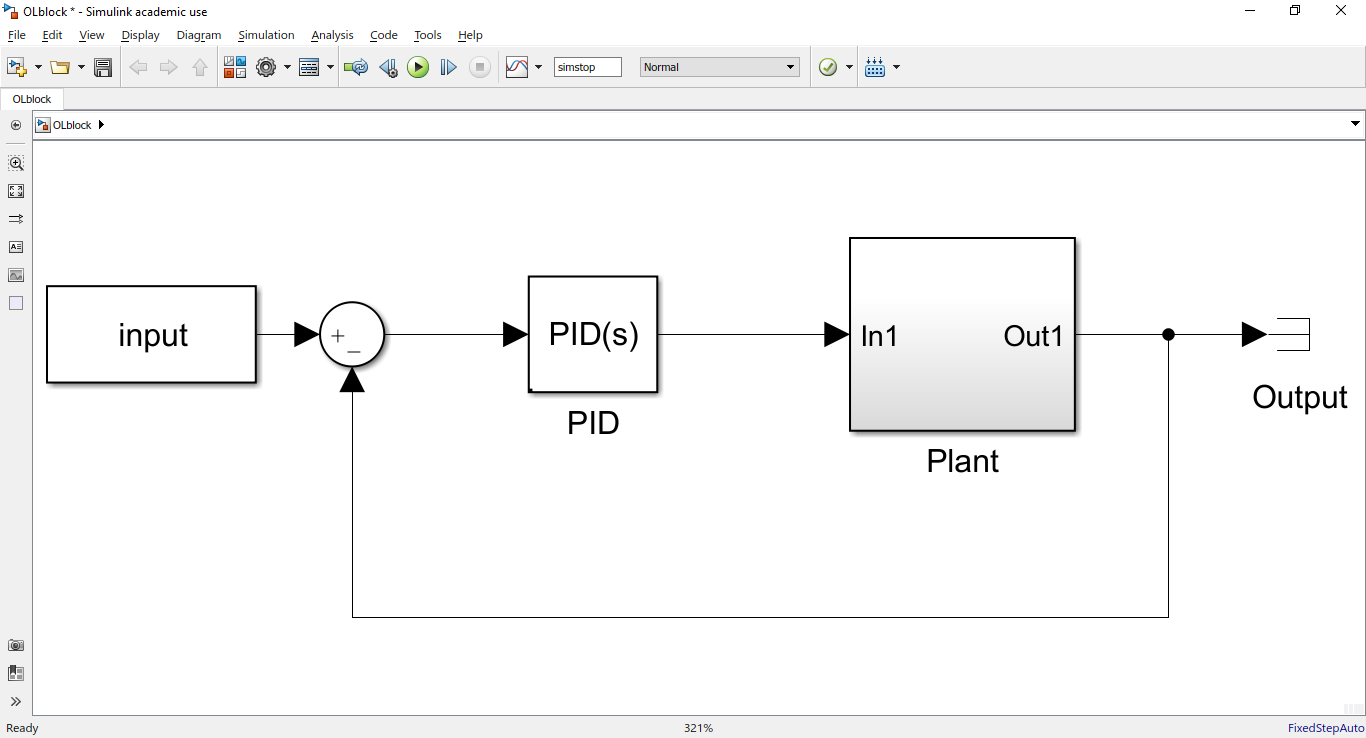
\includegraphics[width=0.75\textwidth]{figures/04ExperimentsAndLabWork/CLblock.png}
    \caption{A simplified block diagram to show the placement of a PID}
	\label{fig:PIDplace}
\end{figure}
\todo[color=05ExperimentsAndLabWork]{crop figure properly}

For the common PID-tuning method as described by Ziegler and Nichols,
some knowledge about the system is needed.
There exist two Ziegler Nichols methods,
depending on the open-loop dynamics of the system.
Because our system has a stable response to a step input, we used the first method described in \todo[color=05ExperimentsAndLabWork]{page 226 ff, Feedback Control of Dynamic Systems}
Here typically a unit step input is given into the OL system as shown in figure \ref{fig:OL}.

\todo[color=05ExperimentsAndLabWork]{get actual values for R and L}
\begin{figure}[H]
    \centering
    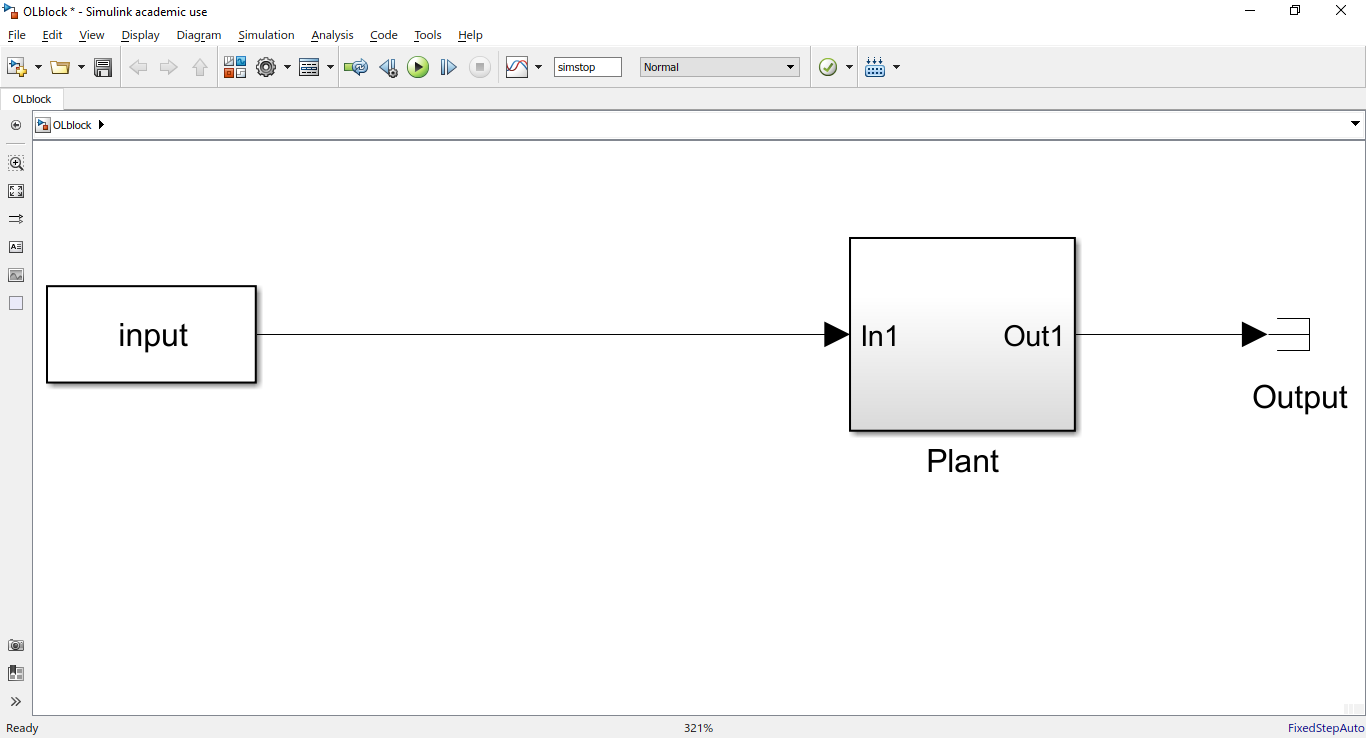
\includegraphics[width=0.75\textwidth]{figures/04ExperimentsAndLabWork/OLblock.png}
    \caption{OL block diagram of the system}
\label{fig:OL}
\end{figure}
\todo[color=05ExperimentsAndLabWork]{crop figure properly}

Because we are scaling the $\omega$ down by a factor of 10, so we can directly read the percentage,
we had to scale the aforementioned unit step up by a factor of 10,
in order to get usable results.
While encountering this problem, we also noticed, that the pumps don't spin below an $\omega$ of 9\%.
When using the corrected step input, we got the measurements shown in figure X \ref{fig:stepin}.

Our analysis of figure \ref{fig:stepin} gives us the following values:
\\
\begin{tabular}{r c l l}
	$A$ 	& $=$ & $2.2177$ 	& \footnotesize{\textit{final value}}\\
	$R$ 	& $=$ & $1.7833$ 	& \footnotesize{\textit{slope}}\\
	$t_d=L$	& $=$ & $0.75$ 		& \footnotesize{\textit{lag}}\\
	$\tau$ 	& $=$ & $1.2436$ 	& \footnotesize{\textit{time constant}}
\end{tabular}
\\
Ziegler-Nichols is tuning a PID controller $D_c(s)$ with the formula\\
$D_c(s)=k_P(1+ \frac{1}{T_Is}+T_Ds)$,
where $k_P$, $T_I$ and $T_D$ are scalar gains,
tuned according to the characteristics obtained from figure \ref{fig:stepin}.

\begin{tabular}{r c l l}
	$k_p$ & $=$ & $\nicefrac{1.2}{RL}$	& \footnotesize{\textit{proportional gain}}\\
	$T_I$ & $=$ & $2L$					& \footnotesize{\textit{integral gain}}\\
	$T_D$ & $=$ & $0.5L$ 				& \footnotesize{\textit{derivative gain}}\\
\end{tabular}


\begin{figure}[H]
    \centering
    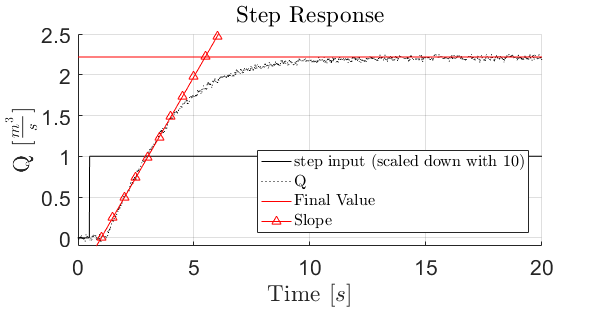
\includegraphics[width=0.75\textwidth]{figures/04ExperimentsAndLabWork/UnitStepResponse1Pump.png}
    \caption{response to a step input with value 10}
	\label{fig:stepin}
\end{figure}
\todo[color=05ExperimentsAndLabWork]{can we make the axis look like they are made by LaTeX as well?}
\\ \\ \\ \\
\todo[color=05ExperimentsAndLabWork]{structure}